\documentclass[pscyr,12pt]{hedlab}
\usepackage[russian]{babel}
\usepackage{graphicx}
\graphicspath{{images/}}

\labname{Установка и настройка веб-сервера IIS, установка MS Visual Studio
  и MS SQL Server}
\labnum{1}
\student{Чечеткин И. А., САПР-1.1п}
\labdate{}

\begin{document}

  \makeheader

  \emph{Цель:} получение практических навыков развертывания инфраструктуры для
  создания Интернет приложений.
  
  \emph{Задание:} развернуть IIS на персональном компьютере и создать
  веб-приложение, отображающее информацию о произвольном предприятии не менее
  чем на пяти страницах, ссылающихся друг на друга. \\

  \emph{Выполнение лабораторной работы:}
  
  \textbf{Предприятие:} ИП "Чоко Пончики".
  
  \textbf{Главная страница:}
  \begin{figure}[h!]
    \center
    
\includegraphics[width=.95\textwidth]{main}
  \end{figure}
  
  \newpage
  
  \textbf{Страница продукции:}
  \begin{figure}[h!]
    \center
    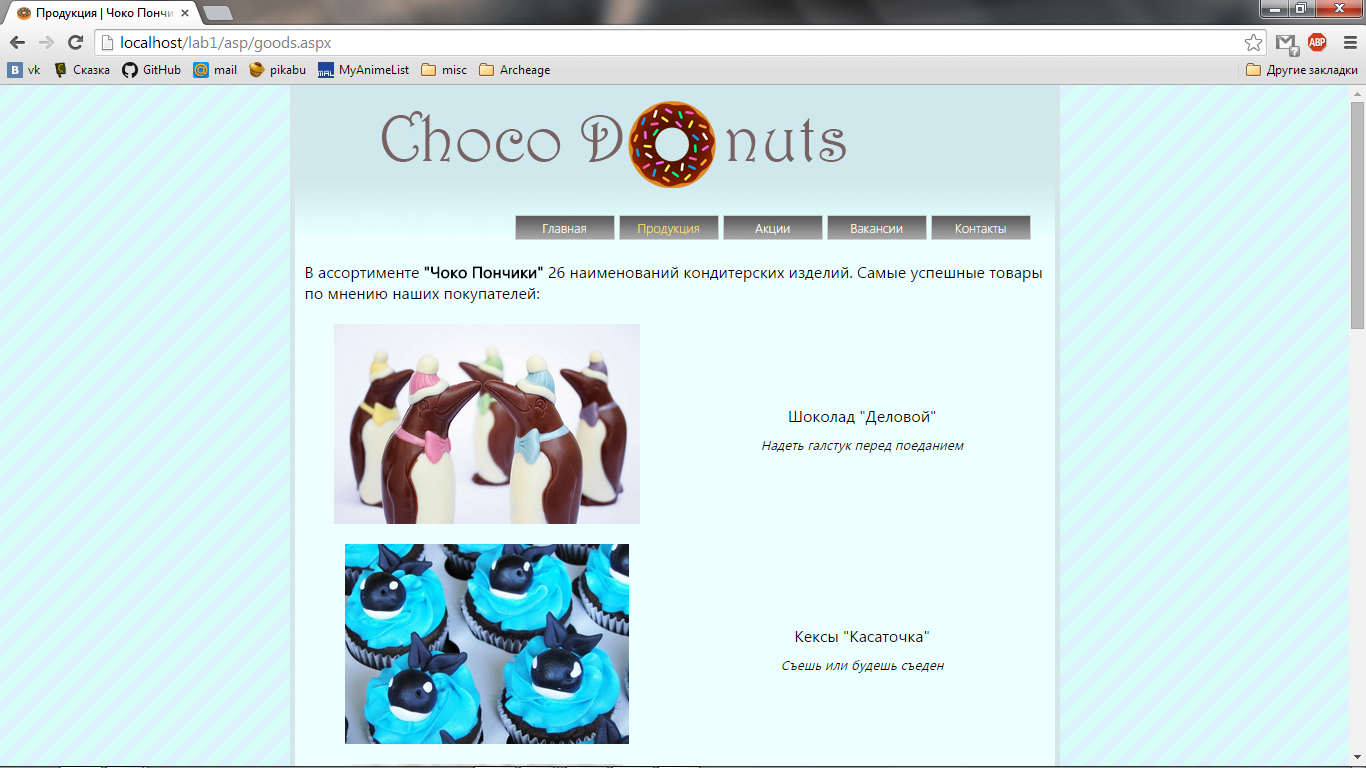
\includegraphics[width=.95\textwidth]{goods}
  \end{figure}
  
  \textbf{Страница акций:}
  \begin{figure}[h!]
    \center
    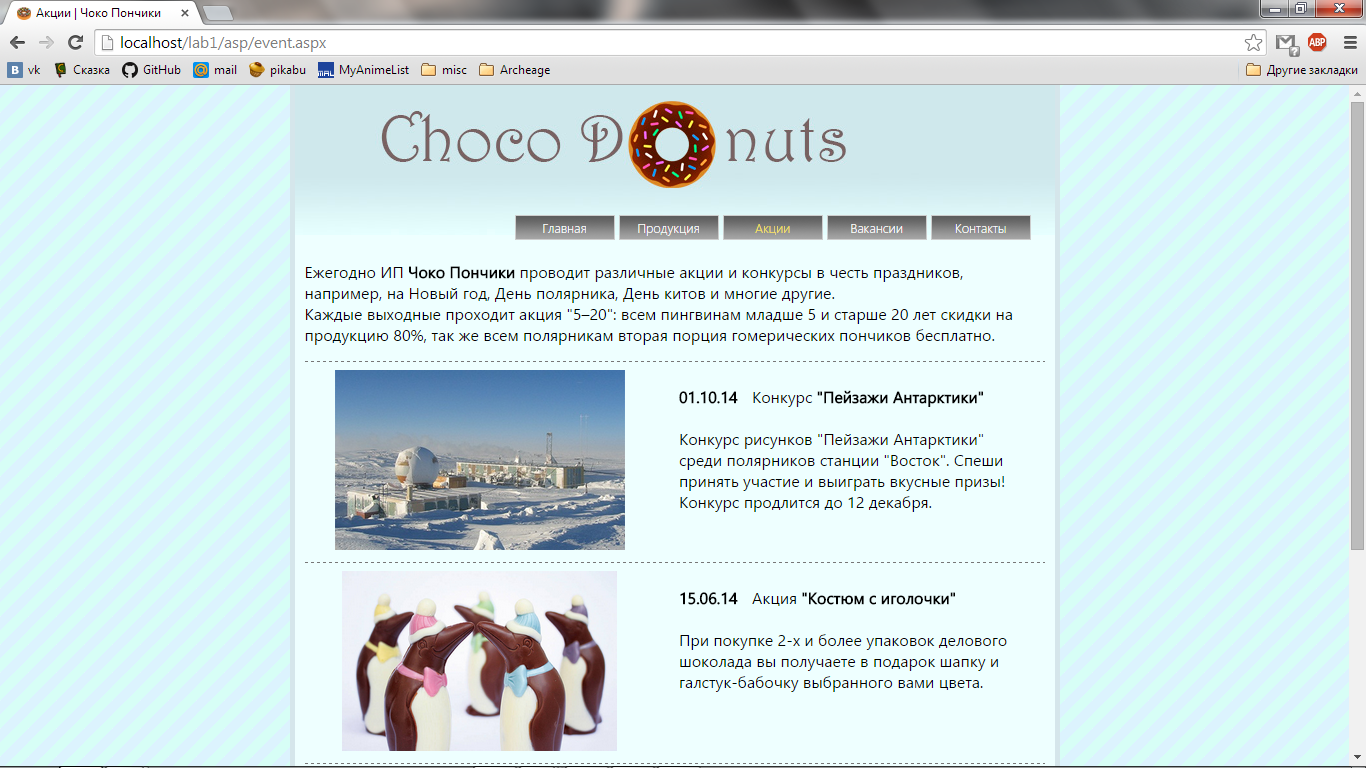
\includegraphics[width=.95\textwidth]{event}
  \end{figure}
  
  \newpage
  
  \textbf{Страница вакансий:}
  \begin{figure}[h!]
    \center
    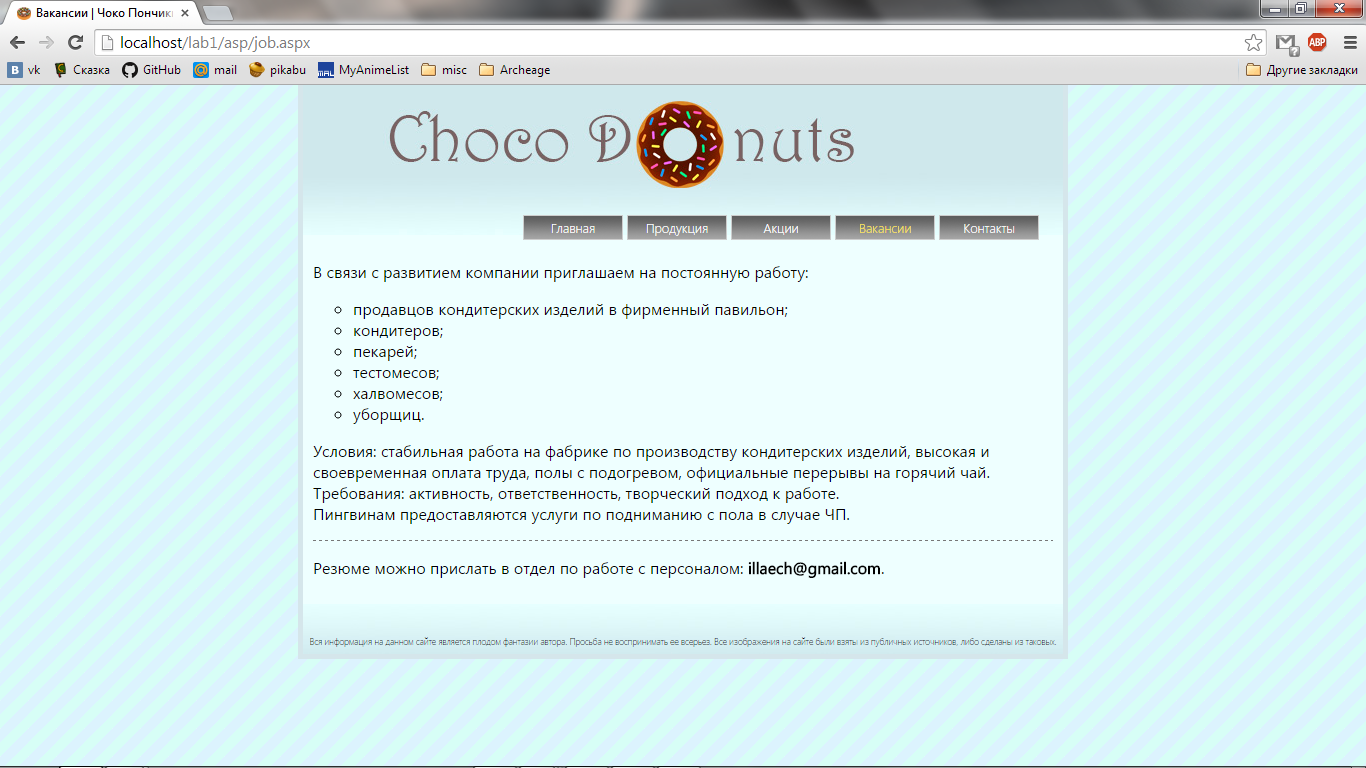
\includegraphics[width=.95\textwidth]{job}
  \end{figure}
  
  \textbf{Страница контактов:}
  \begin{figure}[h!]
    \center
    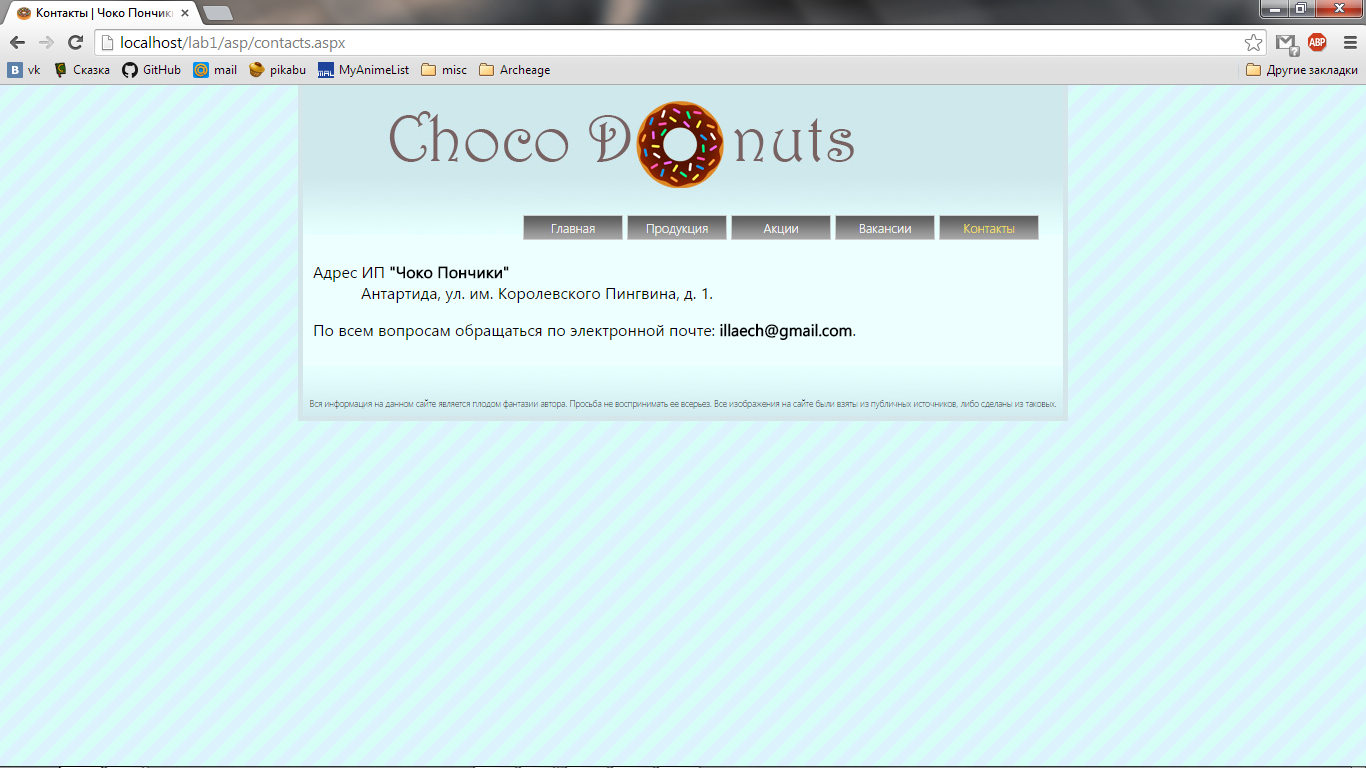
\includegraphics[width=.95\textwidth]{contacts}
  \end{figure}
  
  \emph{Вывод:} в результате проделанной работы
  \begin{enumerate}
    \item установил и настроил веб-сервер Microsoft IIS;
    \item установил инструмент разработки веб-приложений Microsoft Visual
      Studio и СУБД Microsoft SQL Server;
    \item создал и запустил веб-узел.
  \end{enumerate}

\end{document}